\documentclass{capstone}
\usepackage[T1]{fontenc}
\usepackage{parskip}
\usepackage{geometry}
\geometry{margin=2.5cm}
\usepackage{xltabular}
\keepXColumns
\usepackage{array}
\usepackage{bookman}
\usepackage{unnumberedtotoc}
\usepackage{graphicx}
\usepackage[font={small,it}]{caption}
% \usepackage{tabularx}
\renewcommand{\arraystretch}{1.3}
\usepackage{hyperref}
\usepackage{subcaption}
\usepackage{rotating}
\usepackage{amsmath}

\begin{document}

% ------------------ Title Page (no page number) ------------------
\titlepage
	{\includegraphics[width=\paperwidth]{ecse-decal-title}}
	{
		\centering
		{\Large ECSE Capstone Final Report\par}
		\vspace{16pt} 
		{Team 19\par} 	% Replace NUMBER with your team number
		\vspace{16pt}
		{Semester 1, 2025\par} 	% Replace YEAR with the current year
	}

% --- Roman numbering starts here ---
\pagenumbering{Roman}
\tableofcontents
\newpage

% ------------------ Executive Summary ------------------
\addsec{Executive Summary}

This report details the design and implementation of a wireless data acquisition system for EVolocity’s electric vehicle competitions for school children. The system enables real-time wireless transmission of ECU data, eliminating the need for manual retrieval of data by using a USB-C connection. It improves collection accuracy, speed and scalability. The project involved designing a custom ECU, developing embedded firmware and creating a full-stack web application for EVolocity officials to access performance data.

The proposed solution addresses the operational inefficiencies in ECU data handling, enhancing data collection’s speed, accuracy and usability. It features a low-cost, purpose-built solution that exceeds EVolocity’s technical and logistical requirements to streamline competition management and support the programme’s future growth.

The design process involved evaluating various options for wireless communication, user interface design and data syncing strategies. The ideal solution for EVolocity and adherance to the values of Te Tiriti o Waitangi was considered at every stage of the project. The system was implemented with sustainability, digital inclusion and accessibility in mind, by using sustainable suppliers where possible.

The design includes unique features, such as easy setup by upcycling old laptops for the host server, automatic grading, custom event types, mobile-friendly views, zooming on measurements in graphs.

A prototype of the minimum viable product of the system’s hardware, firmware and software components have been built and tested, demonstrating the feasibility of the solution. If this system is adopted, small changes can be made to the hardware and firmware to improve performance, cost, and the software can be extended to support additional features such as user roles and access control. The firmware and software are fully open-source and can be deployed easily.

\newpage

% ------------------ Glossary of Terms ------------------
\addsec{Glossary of Terms}

\begin{table}[h!]
\centering
\begin{tabularx}{\linewidth}{@{}p{2cm}p{4.5cm}X@{}}
\textbf{Acronym} & \textbf{Term} & \textbf{Definition} \\
\\[-1ex]
ADC  & Analogue-to-Digital Converter & A device that converts continuous analogue signals into discrete digital numbers, enabling digital systems to process real-world analogue input like sound or temperature. \\
CRUD & Create, Read, Update, Delete operations & The four basic operations of persistent storage used in databases and software development to manage data effectively. \\
ECU  & EVolocity Control Unit & A custom-built electronic unit used in the EVolocity electric vehicle to measure and record data related to a vehicle’s energy efficiency during races. \\
LED  & Light Emitting Diode & A semiconductor device that emits light when current flows through it. LEDs are widely used for indication, lighting, and display technologies. \\
MVP  & Minimum Viable Product & A product with just enough features to be usable by early adopters, who can then provide feedback for future development. \\
PCB  & Printed Circuit Board & A board used for mounting and connecting electronic components using conductive tracks and pads. \\
RPi  & Raspberry Pi & A small, affordable single-board computer developed to promote computer science education and is often used in prototyping and embedded system projects. \\
SMD  & Surface Mount Device & An electronic component designed to be mounted directly onto the surface of a PCB. \\
SMT  & Surface Mount Technology & A method for producing electronic circuits in which components are mounted directly onto the surface of PCBs, improving manufacturing efficiency and performance. \\
\end{tabularx}
% \caption{Glossary of Technical Terms}
\label{tab:glossary}
\end{table}

\newpage

% % --- Start main content (Arabic page numbers start at 1) ---
\pagenumbering{arabic}
\setcounter{page}{1}


% ################## Introduction ##################
\section{Introduction}

EVolocity’s national electric vehicle competitions aim to inspire the next generation of engineers by engaging students in the design, construction and racing of sustainable transport technologies. A crucial part of these competitions is the collection of performance data from each vehicle’s ECU. However, EVolocity’s current data collection method requires EVolocity officials to manually connect to each ECU via USB-C, which is time-consuming, inefficient and increasingly unsustainable as the number of participants grows.

This report proposes a wireless data acquisition system to resolve these challenges. The system enables real-time transmission of ECU data, eliminating the need for manual retrieval and significantly improving data collection accuracy, speed and scalability. To demonstrate the value of this system, the report presents a business case outlining the client’s needs, key requirements, and the system’s anticipated impact. It then provides a technical overview detailing the design, implementation and integration of the system’s components, supported by testing results and evaluation of key decisions. The report also discusses the project’s outcomes, potential future improvements and how the system aligns with EVolocity’s long-term goals.

By addressing the operational inefficiencies in ECU data handling, this solution enhances data collection’s speed, accuracy and usability and aligns directly with EVolocity’s technical and logistical requirements. Its low-cost, scalable design and tailored software interface present the most suitable solution for enhancing competition management, supporting the programme’s future growth and technological advancement.


% ################## Problem Defintion ##################
\section{Problem Definition}

% ------------------ Project Background ------------------
\subsection{Project Background}

EVolocity is the EV programme inspiring young Kiwis into sustainable engineering while fast-forwarding New Zealand’s clean tech future. Competitions are held annually and involve student teams from intermediate and secondary schools nationwide. Each vehicle is equipped with an ECU that collects performance data such as power consumption and energy usage during races.

Currently, EVolocity officials are required to manually retrieve this data from each vehicle’s ECU by physically connecting to the existing ECU via a USB-C cable. This process must be repeated for each team’s vehicle, which becomes increasingly time-consuming and operationally burdensome as the number of participants grows. Furthermore, delays in data collection can impact event schedules, reducing scoring transparency and adding unnecessary stress to race-day logistics.

This project was initiated to address these inefficiencies and modernise how EVolocity handles race data. Our team has designed a complete wireless data acquisition system with minimal physical interaction, including a custom-built ECU, embedded firmware and a full-stack web application that allows officials to access real-time vehicle performance data with little to no manual intervention. This solution aims to streamline operations, enhance accuracy, and improve the overall competition experience.

% ------------------ Problem Analysis ------------------
\subsection{Problem Analysis}

% ------------------ Initial Problem Statement ------------------
\subsubsection{Initial Problem Statement}

At EVolocity competitions, race officials retrieve data from the ECU of each vehicle manually by connecting to each one via USB-C. The current implementation is time-consuming and inefficient, particularly in fast-paced environments where quick data access is critical. End users, including race officials and event organisers, rely on this data to validate results and ensure fair competition. A wireless system to collect ECU data is needed to streamline this process and improve overall event efficiency.

% ------------------ Discussion ------------------
\subsubsection{Discussion}

In its current form, EVolocity’s data collection process requires EVolocity officials to connect to each vehicle individually using a USB-C cable. This introduces several limitations:

\begin{itemize}
    \item \textbf{Operational efficiency}: With multiple teams competing in a competition, the time spent connecting to each ECU accumulates quickly, resulting in race delays and bottlenecks.
    \item \textbf{Real-time access}: Since data is collected only after a race has concluded, it is not available for live monitoring or rapid decision making.
    \item \textbf{Scalability}: As participation in EVolocity competitions grows, the current system becomes increasingly unsustainable.
\end{itemize}

These challenges undermine the smooth execution of competitions and place unnecessary strain on organisers. Moreover, the lack of automation diminishes the potential for advanced race analytics and performance feedback for student teams.

To address these issues, a new system is needed, one that can collect, transmit and visualise ECU data wirelessly and reliably during or immediately after races.

% ------------------ Evolved Problem Statement ------------------
\subsubsection{Evolved Problem Statement}

The current method of collecting ECU data at EVolocity events, via a manual USB-C connection, is inefficient and time-consuming, resulting in delays, operational overhead and a suboptimal experience for EVolocity officials and participants.

% ------------------ Users ------------------
\subsection{Users}

The primary user group of the system are EVolocity officials. They are responsible for collecting ECU data, validating results and managing competition day operations. Their primary needs are:
\begin{itemize}
    \item Fast and reliable access to vehicle data.
    \item A user-friendly dashboard to manage competitions, events, and teams.
    \item Accurate performance data for scoring and compliance.
    \item A scalable system that simplifies logistics.
    \item A centralised platform for post-event analysis and reporting.
\end{itemize}

% ------------------ Requirements and Critical Success Factors ------------------
\subsection{Requirements and Critical Success Factors}

To ensure the project delivers meaningful value to EVolocity, a set of MVP requirements was established across hardware, firmware and software components. These requirements reflect both technical feasibility and the practical needs of EVolocity officials on competition day. Additionally, several critical success factors were identified to define what constitutes a successful outcome for the system as a whole.

% ------------------ Hardware Requirements ------------------
\subsubsection{Hardware Requirements}

The hardware component of the system is responsible for accurately capturing performance data, specifically voltage and current, from the ECU in real time. It must achieve measurement accuracy within $\pm1\%$ per unit, with a precision of $\pm5\%$ across a batch. The system operates from a standard 12V power source and must include onboard voltage regulation to safely power its internal components. Wireless data transmission is handled by an integrated transceiver, which must reliably operate over a minimum range of 10 meters to accommodate competition-day setups. Additionally, onboard LEDs should provide simple visual feedback to confirm system power and status during deployment.

% ------------------ Firmware Requirements ------------------
\subsubsection{Firmware Requirements}

The firmware, running on a microcontroller, is responsible for sensor data collection, temporary storage, and wireless transmission of sensor data to the server. It should follow a sequential control structure, often referred to as a state machine, to ensure tasks such as data sampling and transmission do not overlap in ways that could affect accuracy. The system is required to stream data at intervals of at least once every five seconds and maintain end-to-end measurement accuracy within $\pm1\%$. 

The firmware must be capable of storing at least one hour of sensor data locally on the microcontroller in situations where immediate transmission is not possible. Once connected to the server, data must be transmitted to the server within five minutes per hour of recorded activity. To ensure reliability in noisy or crowded environments, the firmware includes automatic retry mechanisms for failed transmissions.

% ------------------ Software Requirements ------------------
\subsubsection{Software Requirements}

The software component consists of a backend server and a web-based user interface designed for EVolocity officials to manage competition data efficiently. The interface must support essential functionality such as creating and updating competitions, events, and teams, while also providing access to performance metrics from each team’s ECU.

To support race-day workflows, the software must be mobile-friendly and intuitive, requiring minimal training. It should present data such as voltage, current, and energy usage in a clear and meaningful format, using visual tools like graphs or dashboards. The system must operate reliably over a local network without requiring internet access, while also supporting offline data storage and later syncing with an online database when connectivity is available.

% ------------------ Critical Success Factors ------------------
\subsubsection{Critical Success Factors}

Several factors are critical to the success of the implementation. First, the wireless data transmission must be reliable with automatic retries and minimal data loss, even in noisy, crowded race environments. The system must support concurrent communication with at least 30 ECUs, ensuring it can scale effectively to the number of teams typically present at EVolocity events.

The full data pipeline, from sensor sampling to display on the web interface, must maintain an accuracy within $\pm1\%$ to ensure trustworthy performance metrics. 

The user interface must be simple and intuitive, enabling EVolocity officials to operate the system with minimal training or technical support. To support efficient competition management, ECU data must be transmitted within five minutes of every one hour of recorded activity. 

Finally, the system must be robust and maintainable. It should be well-documented, support modular improvements and scale across multiple teams and competitions without degradation. These qualities are essential to ensure the system remains useful and adaptable beyond the initial deployment.


% ################## Solution ##################
\section{Solution}

% ------------------ Options Considered ------------------
\subsection{Options Considered}

During the early stages of development, several design options were evaluated to determine the most effective approach for collecting and transmitting ECU data in a competition setting.

For wireless communication, the team considered both Bluetooth and Wi-Fi. Bluetooth is commonly used in embedded systems due to its low power consumption and simple pairing process. Wi-Fi, on the other hand, provides higher data throughput and longer range, which are important in environments with many simultaneous devices and potential interference.

When designing the user interface, the team evaluated both mobile-native applications and browser-based dashboards. Mobile apps offer tight integration with specific platforms but introduce development and maintenance overhead, especially when supporting multiple device types. Web-based interfaces, in contrast, can run on any device with a browser and are easier to maintain and deploy, providing a consistent experience across laptops, tablets and phones.

Finally, the team considered different data syncing strategies. One option was to have race officials upload data from each ECU after every race. An alternative approach was to enable automatic syncing whenever an ECU connects to the local network, reducing manual effort and making the system more responsive during competitions.

% ------------------ Initial Options Assessment ------------------
\subsection{Initial Options Assessment}

Each major design decision was assessed based on its suitability for competition-day conditions, operational needs and the long-term maintainability of the system.

Wi-Fi was selected over Bluetooth due to its superior range and performance in multi-device environments. A key project requirement was the ability to support up to 30 ECUs concurrently transmitting data. Bluetooth, while power-efficient and easy to implement, typically supports only 7 to 20 simultaneous connections, well below the required threshold. Wi-Fi, by contrast, can support significantly more connections and provides higher data capacity, ensuring reliable performance in crowded settings.

Rather than building a separate mobile application, the team opted for a responsive web-based interface that works seamlessly on both mobile and desktop browsers. This choice reduces complexity, improves accessibility across a range of devices, and avoids platform-specific compatibility issues, making it easier for EVolocity officials to access the system with the tools they already use.

In terms of data transfer, a post-race upload workflow was considered but ultimately rejected due to its reliance on human intervention. The system instead uses automatic syncing whenever an ECU connects to the server, reducing delays and removing the need for officials to initiate data transfers. This design better supports efficient race management and real-time decision-making.

Overall, the selected options were chosen for their robustness, ease of use, and ability to scale across events, teams, and future deployments.

% ------------------ Economic Assessment ------------------
\subsection{Economic Assessment}

A key advantage of the proposed system is its low cost and scalability, both of which are critical factors for deployment in a nationwide, non-profit, educational program like EVolocity. The project was designed from the outset to be affordable, with component selection and design decisions carefully made to balance performance with budget constraints.

The bill of materials for a single ECU totals approximately \$25.65 when ordered in bulk quantities of 50 units. This includes the microcontroller, voltage and current sensing components, passive elements, and a custom-designed PCB. Compared to commercial telemetry systems, which can cost several hundred dollars per unit, this represents a significant cost saving, especially when scaled across dozens of teams and events.

The firmware and software are fully open-source and custom-built for this application, eliminating the need for recurring licensing fees or third-party platform dependencies. The web interface and backend server are designed to run on local infrastructure, further reducing long-term operating costs and avoiding reliance on paid cloud services.

The software also includes a user-facing event creation feature, enabling officials to define and manage new types of competition-day events directly through the interface. This design choice ensures the system can adapt as EVolocity’s competition structure evolves, without requiring ongoing developer input. By shifting control into the hands of event organisers, the system remains sustainable, flexible and more cost-effective to maintain over time.

Beyond direct financial savings, it also reduces the time and human resources required for manual data collection and scoring. These operational efficiencies translate to indirect economic benefits, such as reduced event overhead and a smoother experience for both officials and participants.

% ------------------ Societal Impact ------------------
\subsection{Societal Impact}

% ------------------ Sustainability ------------------
\subsubsection{Sustainability}

The system was developed with sustainability in mind, both in terms of its physical design and long-term operational impact. EVolocity competitions span schools and regions across Aotearoa, and the ability to reuse, maintain and evolve system components over time helps reduce waste and align with sustainable engineering practices.

A key element of this sustainability strategy is the modularity of the system. Individual components can be replaced or upgraded without requiring a full redesign, which minimises e-waste and repair costs. As the system matures, future EVolocity staff can make incremental improvements, preserving the project’s long-term value and reducing the environmental impact of replacing entire units.

Additionally, the system design reduces hardware wear by avoiding unnecessary writes to flash memory. Since ECU data is transmitted in near-real-time over a local network, there is no need for constant storage on the device itself whilst the ECU is connected to the server. This design choice extends the lifespan of the microcontroller and contributes to the environmental benefits of reduced hardware turnover.

The core firmware is built around the RPi Pico W microcontroller, used in each ECU. This device reflects strong environmental values and supports the sustainability goals of EVolocity. RPi has been awarded the Green Economy Mark in recognition of its sustainable practices and environmental leadership. The Pico W is compact, power-efficient and built for long-term support, making it a responsible choice for embedded systems that are deployed at scale. Raspberry Pi also offers Carbon Removal Credits for customers seeking to offset the environmental footprint of production, shipping and end-of-life disposal of their devices \cite{thornton2025green}.

By combining responsible component selection with modular hardware and efficient local operation, the system supports EVolocity’s broader goals of promoting sustainability and environmental awareness through engineering education.

% ------------------ Digital Inclusion and Accessibility ------------------
\subsubsection{Digital Inclusion and Accessibility}

The system was designed to be accessible across a wide range of devices and usage scenarios, supporting digital inclusion in diverse educational and event environments. By using a web-based interface instead of a platform-specific mobile app, the system can be accessed on any device with a modern browser.

Additionally, the system operates entirely over a local network and does not require an active internet connection to function. This ensures that events held in remote or low-connectivity areas are not disadvantaged and that performance data can still be accessed and managed reliably. This design choice supports equitable access and usability across different regions and resource levels, making the solution more inclusive for all EVolocity officials and organisers.

% ------------------ Te Tiriti o Waitangi ------------------
\subsection{Te Tiriti o Waitangi}

This project incorporates the principles of Te Tiriti o Waitangi through a design process that considers people, place, and environmental responsibility. Māori concepts such as whakapapa, manaakitanga and kaitiakitanga were integrated into the development where appropriate.

The system builds upon the whakapapa of EVolocity’s educational kaupapa and seeks to strengthen whānaungatanga by supporting the effective delivery of competitions nationwide. Accessibility was prioritised through a device-agnostic, offline-capable interface, ensuring an equitable user experience for EVolocity officials, regardless of the location or available infrastructure. This reflects manaakitanga through inclusive design and respect for users’ time, context and capacity.

Environmental sustainability was addressed through modular hardware, power-efficient design, and careful component selection, aligning with the principle of kaitiakitanga. The selection of environmentally responsible components, such as the Raspberry Pi Pico W, further supports this commitment. Surface-mount components were used to reduce material usage and minimise the carbon footprint. The system also reduces waste heat by utilising the microcontroller’s efficient on-board power supply, lowering energy loss to Papatūānuku and helping preserve tapu, New Zealand’s sacred natural resources.

Although formal co-design with Māori communities was not conducted, the development process was user-centred and iterative, reflecting the spirit of mātauranga and tutū. The project is understood as a wero, an opportunity to embed cultural responsibility into technical work and contribute meaningfully to the EVolocity mission.

% ------------------ Best Way Forward ------------------
\subsection{Best Way Forward}

Following a detailed assessment of stakeholder needs, technical feasibility, and long-term value, the proposed wireless data collection system represents the most effective and sustainable solution for improving ECU data handling at EVolocity competitions.

The system consists of three core components:

\begin{itemize}
    \item A custom-designed ECU built around the Raspberry Pi Pico W, capable of accurate data sampling and reliable wireless transmission.
    \item Embedded firmware that ensures end-to-end data integrity, near-real-time syncing, and power-efficient operation.
    \item A web-based interface and backend server that allow EVolocity officials to access competition data, monitor energy performance, and manage events efficiently.
\end{itemize}

This integrated solution eliminates the need for manual data retrieval, significantly reducing delays and labour overhead during events. The web interface is accessible across a wide range of devices and can operate over a local network, ensuring usability even at venues without internet connectivity.

The modular hardware design, low-cost components, and open-source software stack ensure that the system is maintainable and adaptable for future improvements. This makes the solution not only viable for current needs but also capable of supporting EVolocity’s long-term goals around sustainability, growth, and inclusivity.

Adopting this system offers a clear path forward, modernising the competition infrastructure while aligning with EVolocity’s educational and operational values.


% ################## Implementation ##################
\section{Implementation}

% ------------------ Value to EVolocity ------------------
\subsection{Value to EVolocity}

Our wireless data collection system delivers transformative benefits to EVolocity, streamlining competition operations, enhancing event quality, and supporting long-term growth. By addressing the inefficiencies of manual ECU data acquisition, the system empowers EVolocity officials to deliver fair, engaging and efficient competitions

% ------------------ Improved Efficiency and Workflow ------------------
\subsubsection{Improved Efficiency and Workflow}

The system eliminates the time-consuming process of manually connecting to vehicle ECUs via USB-C, reducing data retrieval time to at most 488 seconds for an hour of data. EVolocity officials can access near-real-time ECU data wirelessly, reducing labour-intensive tasks. The user-friendly web interface streamlines data validation and scoring, allowing organisers to focus on race management rather than data entry, significantly improving race-day workflows.

% ------------------ Enhanced Competition Management ------------------
\subsubsection{Enhanced Competition Management}

Wireless data transmission and a tailored dashboard enable officials to access ECU data shortly after each race, improving visibility into energy efficiency, vehicle performance and result validation. This ensures fair competition outcomes, with around $\pm0.8\%$ accuracy, boosting participant trust. Real-time access to performance metrics also streamlines competition-day decision-making and improves the overall experience for organisers. They gain a centralised tool for seamless competition oversight, elevating competition quality.

% ------------------ Scalability and Portability ------------------
\subsubsection{Scalability and Portability}

The system’s PCB and RPi Pico W design supports 50 vehicles across multiple events, accommodating EVolocity’s regional competitions. Its compact, easy-to-install hardware simplifies setup, reducing logistical challenges. The scalable backend server handles growing data volumes, ensuring reliability as competitions expand, making it a versatile solution for EVolocity’s evolving needs.

% ------------------ Future Potential ------------------
\subsubsection{Future Potential}

The system has been developed with modularity and extensibility in mind, providing a strong foundation for further development by EVolicity staff. Several areas of future enhancement have been identified:

\begin{itemize}
    \item \textbf{User Roles and Access Control}: Adding authentication would support a multi-user system, enabling separate interfaces for officials and team participants to view results and leaderboards.
    \item \textbf{Improved Data Storage}: Migrating configuration and logs to external storage such as SPI flash or SD cards would reduce wear on the microcontroller and improve long-term reliability.
    \item \textbf{Firmware Optimisation}: Rewriting performance-critical routines in C/C++ could increase sampling rates, improve energy calculation accuracy and remove Python threading limitations.
    \item \textbf{Hardware Refinement}: The updated PCB design in this report lays the groundwork for future durability, easier mounting and thermal performance improvements.
\end{itemize}

These enhancements would further strengthen the system’s performance, maintainability and alignment with EVolocity’s long-term goals.

% ------------------ Stakeholders ------------------
\subsection{Stakeholders}

\begin{xltabular}{\textwidth}{|l|X|l|X|}
\caption{Stakeholder Analysis Table} \label{tab:Stakeholders} \\
\hline \textbf{Stakeholder} & \textbf{Interest} & \textbf{Influence} & \textbf{Engagement Strategy} \\ \hline
\endfirsthead

\hline \textbf{Stakeholder} & \textbf{Interest} & \textbf{Influence} & \textbf{Engagement Strategy} \\ \hline
\endhead

\hline

EVolocity Officials &
Streamlined data collection, accurate scoring, easy competition management &
High &
Frequent check-ins, testing sessions, requirement validation, demo during development \tabularnewline
\hline

EVolocity Management &
Program scalability, technical viability, cost-efficiency &
High &
Progress reports, cost analysis, long-term sustainability planning \tabularnewline
\hline

Student Teams &
Fair competition, reliable performance data, faster turnaround &
Low &
Indirect engagement via improved systems; future workshops or educational outreach \tabularnewline
\hline

Sponsors &
Positive brand alignment, innovative STEM education, reliable competition &
Medium &
Outcome visibility through improved event execution and data-driven metrics \tabularnewline
\hline

\end{xltabular}


% ------------------ Project Scope ------------------
\subsection{Project Scope}

This project focused on developing a wireless data acquisition system to improve the efficiency and scalability of ECU data collection during EVolocity competitions. The scope of the project included the design, development and testing of integrated firmware and software components.

\subsubsection{In Scope}

\begin{itemize}
    \item Design and assembly of a custom ECU, including a RPi Pico W and supporting sensor circuitry.
    \item Firmware capable of sampling voltage and current at a minimum of 125Hz, storing one hour of data and transmitting it wirelessly.
    \item A local network-based server to receive and store ECU data, with optional syncing to an online database when internet access is available.
    \item A responsive web-based interface for EVolocity officials to manage competitions, view team data and validate performance metrics.
    \item Documentation for system setup, usage and future development.
\end{itemize}
\subsubsection{Out of Scope}
\begin{itemize}
    \item Participant-facing dashboards or authentication-based role separation.
    \item Full-time cloud deployment or reliance on persistent internet connectivity.
    \item Mobile-native applications (the interface is mobile-friendly but browser-based).
    \item Real-time streaming during races (data is only transmitted when the ECU successfully connects to the server).
\end{itemize}
\subsubsection{Constraints}
\begin{itemize}
    \item No reliance on internet connectivity, due to limited infrastructure at competition venues.
    \item Low hardware cost per unit, to ensure affordability at scale.
\end{itemize}


% ------------------ Project Plan ------------------
\subsection{Project Plan}

The project followed a structured timeline across planning, development and testing phases. Figure~\ref{fig:gantt} below outlines the intended schedule.

\begin{figure}
    \centering
    \includegraphics[width=\linewidth]{assets/project-plan.jpg}
    \caption{Gantt Chart demonstrating the planned sequence and duration of tasks.}
    \label{fig:gantt}
\end{figure}

While the project generally adhered to the proposed schedule, minor adjustments were made during the integration phase due to unforeseen delays and iterative improvements to the firmware and software. These adjustments did not affect the delivery of the core system, and all primary deliverables were completed within the final reporting period.

The structured plan helped ensure consistent progress and alignment across sub-teams, while regular check-ins allowed the team to remain adaptive to technical challenges and changing priorities.

% ################## Technical Summary ##################
\section{Technical Overview}

% ------------------ System Overview ------------------
\subsection{System Overview}

Figure~\ref{fig:system-overview} shows the overall system architecture developed for this project. It was built collaboratively by three multidisciplinary teams: hardware, firmware and software. 

\begin{figure}[h!]
    \centering
    \includegraphics[width=0.8\linewidth]{assets/system-overview.png}
    \caption{Detailed system architecture diagram showing the interaction between hardware, firmware, and
software components.}
    \label{fig:system-overview}
\end{figure}

The hardware team was responsible for designing the circuit for voltage and current sensing, including current signal amplification and a step-down linear voltage regulator, the initial and improved designs of the PCB, along with breadboard and PCB-level testing. 

The firmware team developed the embedded software for the RPi Pico W microcontroller, managing accurate sensor data acquisition, digital signal processing, persisting measurements against power losses, and wireless transmission of values to the backend server. 

The software team implemented a backend server that receives data from the ECUs, as well as an intuitive web interface to allow EVolocity officials to efficiently manage the competitions, teams, events and view performance metrics. The data that the ECUs send is stored in a database that is connected to the backend. This data is then displayed by the web interface, along with the other, non-ECU-related data.

% ################## Hardware Design ##################
\subsection{Hardware Design}

Figure~\ref{fig:hw-circuit-design} shows the final circuit design for the hardware component used to measure the voltage and current from the competitors’ vehilces during the competition. The following sections elaborate on the simulation tool used and the components included in the circuit. The component selection further justifies how the components were selected, with attention to alternative options and the value ranges for resistors and capacitors. The PCB design includes an initial design used in the current system, and an improved version of the PCB. Hardware testing goes into detail about the breadboard and PCB testing results after assembly. A cost breakdown of the components used can be found in Appendix~\ref{app:a}.

\begin{figure}[h!]
    \centering
    \includegraphics[width=\linewidth]{assets/hw/hardware-design.png}
    \caption{Overview of Final Circuit Design.}
    \label{fig:hw-circuit-design}
\end{figure}

% ------------------ Circuit Design ------------------
\subsubsection{Circuit Design}

For simulation, LTspice was chosen over PLECS due to its free licensing, extensive online component libraries and greater accessibility. In contrast, PLECS is costly and offers only generic component models, making LTspice the more practical option.

The circuit design, as shown in Figure~\ref{fig:hw-circuit-design} includes current and voltage sensing (Sources and Load), an amplifier for the current sensing signal (Current Sensor Amplification), a LED for debugging (Power LED), a linear voltage regulator (Linear Regulator) and a voltage divider for the ADC reference (ADC Reference) of the RPi Pico W.

Voltage and current sensing circuits must be included for EVolocity to monitor the power used by the competitors’ vehicles during the event. An amplifier must be included for the current sensing signal to convert the analogue signal into a digital signal. According to the datasheet of the RPi Pico W, the ADC range is limited to 0-3.3V, to accomodate this, an operational amplifier was added to the circuit to amplify the current sensing signal to 3.3V.

A voltage divider was added to the circuit for the ADC reference to meet the 3.3V requirement for powering the ADC. Apart from that, the datasheet also suggests using a 5V supply for the RPi Pico W; therefore, a step-down linear regulator was included so that an input voltage of 12V is stepped down to 5V. A Schottky diode was added to prevent excessive current before supplying 5V to the RPi Pico W. To ensure that the circuit is powered with 5V from the linear regulator, an LED was included for debugging purposes.

% ------------------ Component Selection ------------------
\subsubsection{Component Selection}

The linear regulators considered were LD1117V50 and L78L05. To minimise cost, the L78L05 was selected, as it is more cost-effective than the LD1117V50; the L78L05 costs 14.92 NZD for 50 units, whereas the LD1117V50 costs 21.06 NZD for the same quantity. According to the datasheet, the L78L05 provides an output voltage between 4.6V and 5.4V, with a dropout voltage of 2V.

LT6221 and LM324 were evaluated as suitable options for the operational amplifier. Cost was a major consideration in the design of the PCB. The LT6221 costs 386.12NZD for 50 units, while LM324 costs 179.40NZD. Given the 200Hz ADC sampling frequency provided by the firmware, a high slew rate and gain bandwidth were deemed unnecessary; thus, the LM324 was selected. According to the datasheet, LM324 has a unity-gain bandwidth of 1.2MHz and a slew rate of 0.5 V/$\mu$s.

Resistor values within the kilo-ohm range were chosen for most of the circuit to reduce environmental noise and minimise heat after soldering. For the current sensing circuit, 0.1~$\Omega$ shunt resistors with a 3W power rating were chosen to support higher current flow.

For capacitors, an electrolytic capacitor in the microfarad range was used at the output of the linear regulator, serving as a storage capacitor. Ceramic capacitors in the nanofarad range were included for decoupling purposes, as they have lower equivalent series inductance and resistance.

% ------------------ Initial PCB Layout ------------------
\subsubsection {Initial PCB Layout}

For the initial design, the PCB was developed with a focus on cost-effectiveness and environmental sustainability, aligning with Te Tiriti o Waitangi principles of guardianship and the protection of sacred resources. SMT was chosen for the PCB design, as it reduces the carbon footprint, and improves the accuracy and reliability of electronic components compared to through-hole technology.

To minimise waste, the microcontroller was mounted using non-permanent headers, allowing for easy replacement without discarding the entire RPi Pico and ECU unit. Hardware components were selected with long lifespans in mind. The SMT resistors are rated for 1000 hours at temperatures between 68℃ and 72℃. The SMT ceramic capacitors have an estimated lifespan of over 20 years at room temperature, while the electrolytic capacitors, test pins, and female headers have expected lifespans of approximately 10 years.

\begin{figure}[h!]
    \centering
    \includegraphics[width=0.6\linewidth]{assets/hw/initial-pcb.png}
    \caption{Altium render of initial PCB top layer.}
    \label{fig:hw-pcb-top}
\end{figure}

Figure~\ref{fig:hw-pcb-top} shows the PCB layout. The design separates high-power, high-frequency components from low-power signal processing components to minimise noise and interference. High-power, high-frequency components are placed on the right side, while low-power signal processing components occupy the left.

The PCB was also designed for ease of soldering and effective heat dissipation. High-power connections, such as the input, output, shunt resistors and linear regulator, are grouped together and connected through power planes to reduce resistance and noise. Additionally, some interplane capacitance was introduced by using adjacent 5V and ground planes.

% ------------------ Improved Final PCB ------------------
\subsubsection{Improved Final PCB}

Comprehensive feedback from academic experts and internal discussions led to the decision to develop a new PCB Design. This approach was deemed viable, as it significantly reduced the development time that would have been required to modify the existing component placements. The primary issues with the original PCB design were related to the circuit schematic and practical considerations during implementation. 

One of the key flaws identified was the inclusion of a Schottky diode for creating an ORing power supply. This component was ultimately deemed redundant. In this project, the battery power supply consistently provides a higher voltage than the USB power supply, due to a voltage drop across the onboard diode of the RPi Pico W when powered via USB. As a result, the circuit is inherently protected from back current that could potentially damage connected devices (e.g., laptops), thanks to the built-in protection diode on the Pico W itself.

To support this conclusion, a similar power supply circuit was simulated in LTSpice, as shown in Figure~\ref{fig:hw-waveform-of-usb}. The waveform demonstrates that the USB current supply drops immediately after a 5V battery supply is connected to the Pico. The circuit schematic used to produce this simulation can be found in Appendix~\ref{app:b}.

\begin{figure}[h!]
	\centering
	\includegraphics[width=0.9\linewidth]{assets/hw/usb-current-waveform.png}
	\caption{Waveform displaying effects of switching $V_{\text{battery}}$ on and off on the current supply by USB header.}
	\label{fig:hw-waveform-of-usb}
\end{figure}

Another significant issue identified during the PCB review was the obtuse positioning of silkscreen labels (Figure~\ref{fig:hw-obtube-silkscreen}). This was addressed by standardising the orientation of all component labels to the same angle, which facilitates easier soldering and debugging. The improvements made to silkscreen positioning are illustrated in Figure~\ref{fig:hw-correct-silkscreen}.

\begin{figure}[h!]
    \centering
    \begin{subfigure}[b]{0.45\textwidth}
	\centering
	\includegraphics[width=0.8\linewidth]{assets/hw/obtuse-silkscreen.png}
	\caption{Example showing obtuse label orientations.}
	\label{fig:hw-obtube-silkscreen}
\end{subfigure}
\hfill
    \begin{subfigure}[b]{0.45\textwidth}
	\centering
	\includegraphics[width=0.8\linewidth]{assets/hw/correct-silkscreen.png}
	\caption{Example showing updated component label orientations.}
	\label{fig:hw-correct-silkscreen}
    \end{subfigure}
    \caption{Examples of obtuse and corrected silkscreen.}
\end{figure}

A critical post-manufacturing issue involved floating inputs on two operational amplifiers within the LM324 SOIC-14 package. This problem was mitigated by repurposing the unused op-amp channels as buffers for the voltage sensor, current sensor, and ADC reference. Leaving op amps powered with floating inputs can lead to unwanted amplification of environmental noise, resulting in both unstable signal behaviour and unnecessary power dissipation. A commonly recommended solution is to ground the non-inverting input and connect the inverting input to the output to create a negative feedback loop \cite{working-opamp}. Figures~\ref{fig:hw-floating-opamp-inputs} and \ref{fig:hw-utilised-opamp-inputs} illustrate the changes made to resolve this issue.

\begin{figure}[h!]
    \centering
    \begin{subfigure}[b]{0.45\textwidth}
	\centering
	\includegraphics[width=\linewidth]{assets/hw/floating-opamp-inputs.png}
	\caption{Example displaying floating opamp inputs.}
	\label{fig:hw-floating-opamp-inputs}
\end{subfigure}
\hfill
    \begin{subfigure}[b]{0.45\textwidth}
	\centering
	\includegraphics[width=\linewidth]{assets/hw/utilised-opamp-inputs.png}
	\caption{Example of utilised op amp pins.}
	\label{fig:hw-utilised-opamp-inputs}
    \end{subfigure}
    \caption{Example displaying utilised opamp input ports.}
\end{figure}

Thermal relief was another concern, as poor thermal design can lead to tombstoning and cold solder joints. The initial PCB design had areas with uneven copper pour connections, and certain resistors were placed too closely together. These conditions increase the risk of tombstoning, where one end of an SMD component lifts off the board due to imbalanced solder wetting. This occurs when heat flows unevenly between the solder pads, causing one end to reflow faster than the other. Figures~\ref{fig:hw-unveven-copper} and \ref{fig:hw-even-copper} show a visual comparison of a problematic layout and the corrected version. The final (fourth) PCB revision addressed these thermal issues in two main ways. Firstly, resistor spacing was increased to prevent heat from rapidly transferring between adjacent components during soldering. Secondly, a design rule was introduced to enforce a minimum polygon plane trace width of 1.5mm, ensuring more uniform thermal distribution across the board.

\begin{figure}[htbp]
    \centering
    \begin{subfigure}[b]{0.45\textwidth}
	\centering
	\includegraphics[width=0.7\linewidth]{assets/hw/uneven-copper-connections.png}
	\caption{Example showing uneven copper connections on both sides of components C4 and R8.}
	\label{fig:hw-unveven-copper}
\end{subfigure}
\hfill
    \begin{subfigure}[b]{0.45\textwidth}
	\centering
	\includegraphics[width=0.7\linewidth]{assets/hw/even-copper-connections.png}
	\caption{Example showing evenly spaced out connections between resistors in the final revision of PCB.}
	\label{fig:hw-even-copper}
    \end{subfigure}
    \caption{Examples of uneven and even copper pours.}
\end{figure}

% ------------------ Hardware Testing ------------------
\subsubsection{Hardware Testing}

Two phases of testing were conducted: breadboard testing and PCB testing. Breadboard testing served as an initial prototyping stage, allowing the team to validate the design, debug circuit behaviour, and refine component values based on theoretical calculations. This phase was essential for identifying and correcting issues before committing to a PCB layout.

PCB testing followed the assembly of the final circuit and focused on verifying performance after soldering. It assessed the accuracy and reliability of the assembled components. If necessary, further adjustments to component values were made at this stage to optimise the circuit’s performance.

% ------------------ Breadboard Testing ------------------
\subsubsection{Breadboard Testing}

\begin{figure}[h!]
    \centering
    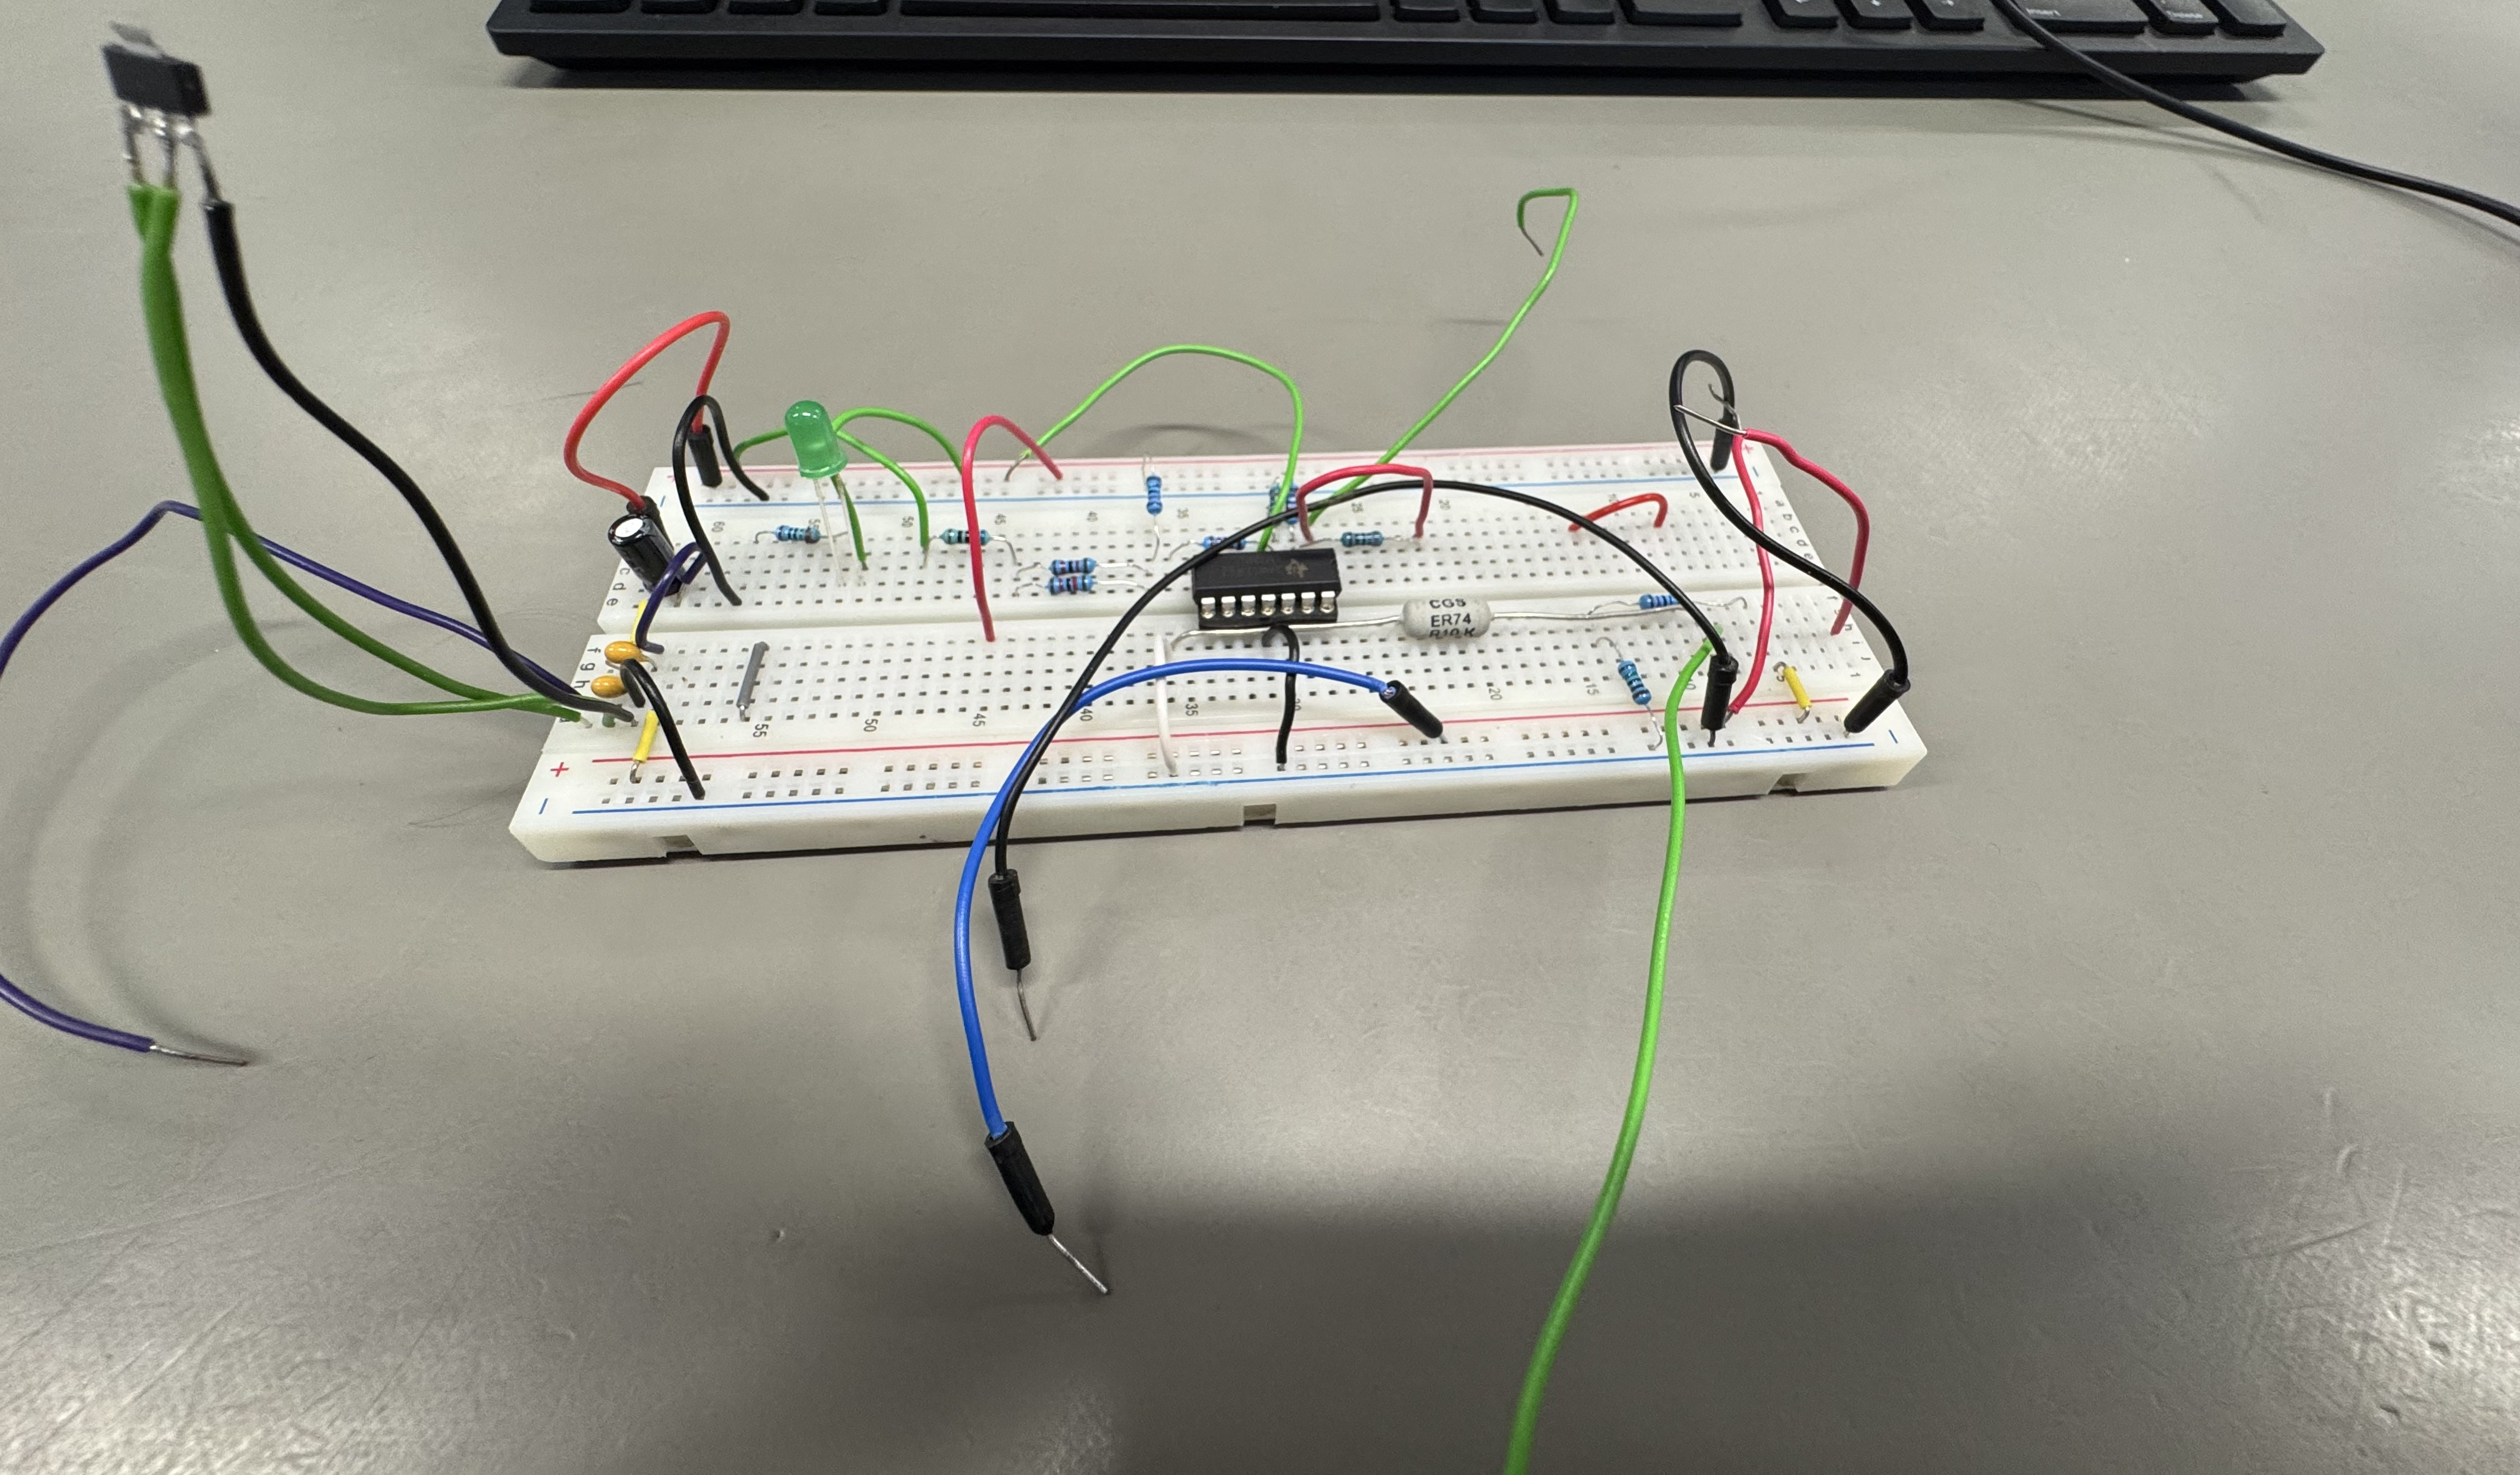
\includegraphics[width=0.6\linewidth]{assets/hw/breadboard.png}
    \caption{Breadboard used for testing}
    \label{fig:hw-breadboard}
\end{figure}

Figure~\ref{fig:hw-breadboard} shows the breadboard setup used for initial testing. The breadboard was used to validate the circuit design before soldering the components onto the PCB. Testing confirmed that the output signals closely matched the simulated results and exhibited minimal noise.

An oscilloscope was used to probe key signals, including the output of the voltage regulator and the voltage supply for the ADC reference. These measurements are shown in Figures~\ref{fig:hw-regulator-output} and~\ref{fig:hw-adc-output}. Additionally, Figure~\ref{fig:hw-breadboard-sensor-tests} presents the observed signals for voltage sensing and current sensing.

\begin{figure}[h!]
    \centering
    \begin{subfigure}[b]{0.45\linewidth}
        \centering
        \includegraphics[width=\linewidth]{assets/hw/regulator-output.png}
        \caption{Output of voltage regulator tested on breadboard.}
        \label{fig:hw-regulator-output}
    \end{subfigure}
    \hfill
    \begin{subfigure}[b]{0.45\linewidth}
        \centering
        \includegraphics[width=\linewidth]{assets/hw/adc-output.png}
        \caption{Output of ADC reference tested on the breadboard.}
        \label{fig:hw-adc-output}
    \end{subfigure}
    \caption{Breadboard testing outputs for the voltage regulator and ADC reference.}
    \label{fig:hw-breadboard-testing}
\end{figure}

\begin{figure}[h!]
    \centering
    \includegraphics[width=0.5\linewidth]{assets/hw/breadboard-sensor-tests.png}
    \caption{Voltage and Current sensor values tested on the breadboard.}
    \label{fig:hw-breadboard-sensor-tests}
\end{figure}

Following PCB assembly, testing was conducted to verify functionality and compliance with design specifications. In the absence of an EVolocity car, a realistic load profile based on Formula 1 race data was used to simulate dynamic driving conditions. 

The 5V regulator was evaluated under load to provide a stable output with minimal ripple. The current drawn through the debugging LED, connected to the regulator, was measured at 19mA, which is well below the LED’s maximum DC forward current, ensuring reliable operation and long lifespan.

\begin{figure}[h!]
    \centering
    \begin{subfigure}[b]{0.45\linewidth}
        \centering
        \includegraphics[width=\linewidth]{assets/hw/current-reading.png}
        \caption{Current sensor readings.}
        \label{fig:hw-current-reading}
    \end{subfigure}
    \hfill
    \begin{subfigure}[b]{0.45\linewidth}
        \centering
        \includegraphics[width=\linewidth]{assets/hw/voltage-reading.png}
        \caption{Voltage sensor readings.}
        \label{fig:hw-voltage-reading}
    \end{subfigure}
    \caption{Voltage and current sensor oscilloscope readings from the PCB.}
    \label{fig:hw-voltage-current-readings}
\end{figure}

\begin{figure}[h!]
    \centering
    \includegraphics[width=0.5\linewidth]{assets/hw/load-test.png}
    \caption{Realistic load used to test the PCB}
    \label{fig:hw-load-test}
\end{figure}

Figure~\ref{fig:hw-voltage-current-readings} illustrates how the sensed voltage and current values respond to the dynamic load shown in Figure~\ref{fig:hw-load-test}. The measured voltage remained relatively stable around 1.5V (1.495V-1.573V). The voltage representing the sensed current varied between -0.121V and 1.085V, which provides a suitable range for monitoring current fluctuations without any signal clipping.

% ################## Firmware Development ##################
\subsection{Firmware Development}

The primary objective of the firmware is to implement a robust system for collecting, storing, processing, and transmitting the values measured by the hardware. To achieve this goal, the voltage and current are periodically sampled, along with timestamps. A signal processing state calculates the energy and average values from the high sample rate into smaller amounts of information, and the data is streamed to the server or stored to flash, depending on whether a connection with the server is active, as per the firmware system data flow diagram (Figure~\ref{fig:fw-overview}).

\begin{figure}[h!]
    \centering
    \includegraphics[width=0.8\linewidth]{assets/fw/overview.png}
    \caption{Flow of data through the firmware, from sampling to processing and transmission.}
    \label{fig:fw-overview}
\end{figure}

% ------------------ Firmware Techonologies ------------------
\addsubsubsec{Firmware Techonologies}

% The  chosen microcontroller was the Raspberry Pi Pico W microcontroller board, as it aligns treaty values with ethical sourcing, availability, fast lead time, class-leading sustainability, and low cost (\$10) through official channels. The Raspberry Pi Foundation leads commitments for energy-efficient computing, product longevity (through good quality hardware, documentation and long-term software support), and reducing/mitigating their carbon footprint across the lifecycle of their product.

With the commitment to making the solution open and inclusive and aligning with the treaty principles of partnership, MicroPython has been picked as our development language for the firmware. Python is commonly taught in schools and is one of the most common programming languages, with 51\% of developers employing this language \cite{python-stat}. MicroPython allows for easily adding modularity to the firmware, improving readability without the complexity of CMake files. It also abstracts more complex peripheral register setup code, making it more accessible to school children. MicroPython APIs transparently bring improvements over raw C APIs, including utilising LittleFS, a file system designed for microcontroller flash applications with bounded/limited resource usage. Copy-on-write techniques are used to ensure resilience against random power losses. It also implements dynamic wear levelling and works around bad blocks. An annotation can enable the native code compiler or Viper compiler to generate optimised bytecode to improve performance.

% ------------------ Sensor Measurement ------------------
\subsubsection{Sensor Measurement}

The first step of the firmware is to sample the signals from the hardware using Pico's ADCs. The inputs are connected through pins GPIO26 and GPIO28 to measure voltage and current, respectively.

To ensure accurate timing, the Pico's Programmable Input/Output (PIO) was used with a custom assembly program to generate interrupts at a precise rate of 200Hz, independent of the software running on the processor cores. This improves performance over purely software-based timers, which will jitter or be indeterminate based on the current workload on the cores. A deviation to the overall program state machine logic was added after the proposed design; the implementation moved away from state machines, where sampling was stopped during data upload. ADC readings will now be continuously captured, even during uploads. This implementation allows for continuous streaming to the server if the race track is small and the ECU remains connected, while ensuring that the power limit can be continuously monitored. The measured ADC values are packed into a four-byte float instead of a Python-native float to improve memory efficiency and ease optimisation for the native code/Viper compiler for calculations.

% ------------------ Data Packing into Compact Binary Format ------------------
\subsubsection{Data Packing into Compact Binary Format}

After sampling and signal processing, the results are packed into a compact binary format and placed into a queue for the data transmission task. To improve memory efficiency and flash usage, the values remain packed in the compact binary format for the remainder of the time they are handled on the Pico. The calculation and packing functions are optimised using the MicroPython Viper Native compiler, which allows MicroPython to compile the code to bytecode, improving performance for packing and unpacking data. Operating on Viper-native datatypes greatly improves performance, and in our tests, the overhead of conversion from a Python-native data-type is justified for compute-heavy functions.

% ------------------ Digital Signal Processing (DSP) ------------------
\subsubsection{Digital Signal Processing (DSP)}

To avoid overloading the flash and backend with measurements and to improve accuracy, samples are batched into larger groups and unpacked. Key metrics, including the peak values and averages, are calculated, and the sample's timestamp is bundled with the data. Using this information, the software team can easily create a solution that can display the energy, power, current, and voltage usage with respect to time while ensuring that cars exceeding the power limits can be noted and penalised.

The signal processing task is run on a separate core to ensure that long computation times do not interfere with data uploading and that the sampling ISRs do not interfere with the signal processing. Thread-safe queue data structures are used for communication between the main task on core zero and the processing task on core one. The processing converts raw ADC values of the current and voltage to more accurate Volts and Amperes, alongside power calculation and energy calculations. Once 10 samples are connected for each, the average voltage, current, and power are calculated, along with the peak values for power. The energy calculations are performed on the microcontroller to obtain the total energy consumption, to allow for high confidence in the precision of the timing of readings.

The ADC RP2040 microcontroller used by the Pico contains an unfixable hardware bug/errata (RP2040-E11) \cite{rp2040_datasheet} due to incorrect capacitor choices inside the microcontroller's ADC's successive approximation circuit, causing severe differential nonlinearity spikes. This is exhibited by jumps/discontinuities in ADC measurements, as can be seen in the red points in Figure~\ref{fig:hw-calibration}. To mask the effects of this, a calibration profile with different weights for each bit can be applied as shown in Appendix~\ref{app:c}, as shown by the blue points.

\begin{figure}[h!]
    \centering
    \includegraphics[width=0.6\linewidth]{assets/fw/calibration-line.png}
    \caption{Raw vs actual current measurements from test load and ADC. Red points show raw ADC values, blue points show calibrated values.}
    \label{fig:hw-calibration}
\end{figure}

The measured voltage and current are then scaled using the simulation results from the hardware to calculate the true voltage and current values.

% ------------------ Network Connectivity and Data Upload ------------------
\subsubsection{Network Connectivity and Data Upload}
The ECU attempts to connect to Wi-Fi and upload values to the server every five seconds. The onboard LED is used as a status indicator to show the status of the connection. A solid light indicates that the Pico is connected to the server, a slow blinking light indicates the ECU is connecting to Wi-Fi, and rapid blinking indicates the ECU is attempting to discover the backend server on the local area network.

The ECU attempts to connect to a hotspot hosted on a phone or the device hosting the server and then tries to discover the server's IP address. The server emits a UDP broadcast beacon packet on a predetermined port every 250ms, which the ECUs listen for. Once the IP address is obtained, the ECUs check if the server is our official server by checking a predetermined endpoint.

After connecting to the server, the ECU checks for the backlog of measurements stored on the flash that have not been uploaded to the server and performs a streaming upload (detailed in Section~\ref{sec:measurement-and-configuration-storage}). If no backlog exists and the server's connection is healthy, the ECU batches measurements from the previous calculations stage into STREAMING\_BATCH\_SIZE chunks to transmit to the server at once. Batching reduces the backend load and the ratio of CPU time spent on the overhead of requests to the time spent handling data transmission.

As the data is only stored in memory as a buffer, it is not written to disk, provided that the connection to the server is stable, allowing the solution to prolong the life of the flash's hardware. If the connection to the server is lost, measurements will be written to flash.

The ECUs and servers communicate over HTTP over TCP/IP. TCP implements error detection, handling and retransmission, allowing for guarantees that the measurements are transmitted correctly. HTTPS introduces significant overhead in both memory usage and compute overhead on the firmware. HTTPS and SSL encryption are unnecessary as WPA2 authentication used by the Wi-Fi access point utilises a four-way handshake to establish an encrypted connection between ECUs and the host server, ensuring that packets cannot be spoofed or sniffed.

A broadcasting feature was also implemented to allow the Pico to broadcast its serial number to the server to identify itself when the button is held after the Pico is power-cycled.

% ------------------ Measurement and Configuration Storage ------------------
\subsubsection{Measurement and Configuration Storage} \label{sec:measurement-and-configuration-storage}

The Pico's flash is known to be prone to corruption on power loss and has limited write endurance. The firmware employs some mitigations, such as using LittleFS, but it is also designed to write as little as possible to the flash. With only the Session ID and serial number stored on the flash, the firmware is almost stateless across power cycles and is resilient to power losses. The serial number is obtained from the MAC address of the Pico, and it is stored in flash to allow for changing the value, but it is discouraged. The session IDs are incremented every time the ECU is turned on. Upon resetting, the software can handle duplicate session IDs by incrementing them to the next available session ID value.

JSON is used to store persistent configuration data, including the session\_id and pico\_id, to balance small file size and human readability. File system operations are cached to improve performance and reduce wear on the flash. This is done to allow caching values where possible to reduce the number of flash read/write operations. The Pico's default ID is its MAC address, which is unique per Pico and does not require changing.

As the Wi-Fi connection may drop during the race, measurements must be persisted to the flash in case of a power failure whilst out of range. A binary file stores the packed values from the signal processing phase. We append the batches of measurements to the end of the file. A free space check is performed before writing to the flash.

As the measurement protocol is the same as the previously packed values, the files can be streamed from the file as-is in chunks without loading the entire file into memory for transformation. Due to the nature of MicroPython's memory allocations, memory may become fragmented, meaning that whilst a large amount of memory may be free, contiguous memory blocks may be unavailable. Opportunistic dynamic chunk sizing during runtime is implemented to increase the amount of data chunked to up to 500 readings at once, provided that there is enough free continuous memory. Chunk streaming will allow efficient uploading of large measurement backlogs in chunks, reduce memory overhead whilst uploading, and allow more measurements to be uploaded compared to other formats, such as JSON.

% ------------------ Firmware Simulations, Implementation, and Testing ------------------
\subsubsection{Firmware Simulations, Implementation, and Testing}

Before implementing the firmware, the firmware was tested in simulators to ensure each part of the required functionality in the MVP, such as ADC sampling, storage and transmission, would be met. Initial testing scripts written in Wokwi (Appendix~\ref{app:d}) used both C and MicroPython to evaluate the performance of the different language options. The simulation was done to ensure that the program continues working whilst adding new functionality.

Initially, a simple ADC capture loop was simulated and tested on the physical board. A simple function was implemented to capture the raw ADC value and convert it to a float of the corresponding input voltage. In the next iteration, chunking, along with a CRC32 checksum, was implemented. Checksum validation is a process used to ensure that a file or data block has not been altered or corrupted during transmission or storage.

After each driver was written and tested to run as expected in the simulator, the tasks were made to work concurrently with the \texttt{asyncio} library.

To test the integration of the firmware before the software was completed, a mock server was created to take in values from the firmware and calculate the energy consumption of the load and the recorded values. The mock server also served as a reference implementation for decoding the binary format.

For verification against the range of values, the mock server was modified to control and read the Virtual Instrument Software Architecture (VISA) protocol from the load to compare the sampled value against the actual values. The measured current against the read current of a sweep of resistances is logged to a file and plotted onto Desmos in Appendix~\ref{app:e}. The firmware's performance remained constant when we conducted additional measurements after swapping our Pico for an alternative unit.

% https://discord.com/channels/1346668640300433510/1347409835401941004/1376041558801125379
% Caption: Testing code to store values showing the implementation of chunking and CRC32 checksum validation.
% [THIS LOG IMAGE IS NOT USEFUL; CAN BE DELETED IF PRESSED FOR SPACE

% ------------------ Firmware Improvements ------------------
\subsubsection{Firmware Improvements}
The most common point of failure with our hardware design was the RPi Pico W. By using female headers instead of soldering the RPi Pico to the board, we have made it easy to swap out. However, the flash is still prone to wearing out. Writing the configuration and measurements to an external SPI flash or an SD card will prolong the lifespan of the Pico.

Our sampling rate of 200 Hz can be further increased with further optimisations to the calculation code to improve the accuracy of our energy calculations. A rewrite in C/C++ may improve performance and bring additional benefits, allowing lower-level control over the hardware and allowing the hardware timers to be used. In addition, the Python Global Interpreter Lock hinders the full potential of multithreading with Python, which will not be the case with a C/C++ implementation.

% ################## Software Implementation ##################
\subsection{Software Implementation}

% ------------------ Frontend Architecture and Design Goals ------------------
\subsubsection{Frontend Architecture and Design Goals}

The frontend was created in React using TypeScript and is designed to run smoothly on any modern browser for any phone or laptop. The goal was to create a simple, no-fuss user interface that was easy to use. Since the users are likely to be volunteers, they won’t have time to learn a complicated system, and they won’t be looking for a flashy, visually stimulating interface—they want a pain-free scoring experience so they can focus on attending to the events and teams.

Thus, the frontend consists of three simple pages: a competitions, teams, and event types page—each for managing their respective areas. The application begins at the homepage, which contains links for each page, and there is a navigation bar at the top of every subsequent page for ease of navigation. The application does not include a login screen, as it will only be run by the EVolocity scoring team. Adding a login would create unnecessary steps for users at this stage. A comparison of the initial and final design of the UI can be found in Appendix~\ref{app:f}.

% ------------------ Feature Overview and Improvements} ------------------
\subsubsection{Feature Overview and Improvements}

The functionality of the website is as follows:

\begin{itemize}
  \item \textbf{Manage Teams}: Users can create, edit, and view teams. This includes team names, vehicle class, and vehicle type.
  \item \textbf{Assign Team to ECU}: Users can match a team to its device serial number—thus linking the two for scoring. The serial number is 3D printed on each ECU for easy access. When a team presses their Pico’s Wi-Fi button, the web application displays a real-time notification with the serial number of the pressed device. This allows volunteers to easily map teams to ECUs.
  \item \textbf{Manage Event Types}: Users can create, edit, and view events. This allows future event changes to be made directly through the UI rather than through code.
  \item \textbf{Manage Competitions}: Users can create, edit, and view competitions. When creating a competition, users can set the name, select at least three events, and assign at least one team. Teams can also be created here if they were missed earlier. If the user is online, they can also load and view past competitions.
  \item \textbf{Scoring and Leaderboards}: After each event is completed, users can press the ‘Finish and Score’ button to display the leaderboard for that event by vehicle category (e.g. Open Kart, Standard Bike, etc). An overall leaderboard is also maintained and updated as events are scored.
  \item \textbf{ECU Monitor}: The ECU displays three graphs for voltage, current, and energy. Hovering over each graph shows more detailed measurement data.
\end{itemize}

% ------------------ User Flow for Race Day ------------------
\subsubsection{User Flow for Race Day}

The final user flow diagram, Figure~\ref{fig:sw-user-flow}, includes updated steps to reflect changes in functionality:

\begin{figure}[h!]
    \centering
    \includegraphics[width=\textwidth]{assets/sw/user-flow-diagram.png}
    \caption{Updated user flow diagram reflecting team-to-ECU assignment and simplified scoring path.}
    \label{fig:sw-user-flow}
\end{figure}

\begin{itemize}
  \item Add team-to-ECU assignment
  \item Add team creation within competition creation
  \item Add scoring and retry scoring
  \item Remove “connect ECUs per event”
\end{itemize}

Team-to-ECU assignment can happen at any point until scoring. Assuming all teams are registered with their vehicle details, the team, event, and competition setup can be done before race day. Then, on the day, users simply assign ECUs and press the ‘Score and Finish’ button per event, making the workflow as efficient as possible.

% ------------------ Backend Architecture and API Design ------------------
\subsubsection{Backend Architecture and API Design}

The backend was developed using Supabase for the cloud database, while a local SQLite database was used during events to allow offline operation. It is paired with Docker to ensure reliable and uniform deployment regardless of the environment. We have a robust API layer which connects Next.js and Supabase through Prisma. This allows seamless communication between the frontend interface, ECUs and the database. We chose these technologies to accommodate rapid development, reliability, and straightforward deployment.

The backend architecture uses a RESTful API structure and standard HTTP methods, including GET, POST, PATCH, and DELETE. Each endpoint was created for a specific resource for the application, including teams, devices, competitions, races, and sensor data. This structure allows for predictable and reliable interactions between different system components, essential for a multi-disciplinary system. A full list of the API routes can be found in Appendix~\ref{app:g}.

All API routes were structured using JSON formats and standard HTTP status codes to help with debugging and communication between backend and frontend components. Error handling and validation were implemented to help reduce the risk of failures due to malformed data inputs.

API endpoints were created for every relation only where necessary. Instead of having CRUD for every object type we only made the endpoints where needed (or would be needed in future). This created a simpler backend that does not have unused routes. There are also additional endpoints that are not from the schema, which are specialised for device assignment and device handshaking. These also ensure that in addition to wifi connectivity, the actual server is also online.

% ------------------ Database Management and Offline Operation ------------------
\subsubsection{Database Management and Offline Operation}

The cloud database uses Supabase, which is a PostgreSQL-based platform. For local usage, a lightweight SQLite database was used. Both shared the same schema structure, which made it straightforward to test and sync data between local and cloud environments. The defined schema contains models for race, event, competition, ranking, team, device, device configuration, record, sensor data, and notification. 

Prisma was used during development to inspect and manage the database contents. Prisma allows a level of abstraction between raw SQL code (used with both Supabase for cloud and SQLite for local) and the Next.js backend. This made testing and development easier across both environments. Pushing the schema through Prisma and using a seed script to populate the database with test data allowed for an easy development pipeline.

Due to the client's anticipation of unreliable internet connection during race day events, the backend was designed with offline-first and online connectivity functionality if available. A local SQLite instance was put into a Docker container and will run entirely on the laptop used on race day. All core functionality works without internet access. Data generated during events will be stored in the local SQLite database. The data can then be uploaded to the cloud through the API/sync endpoint. The user manually triggers this via a button on the frontend once they have an internet connection.

A manual database syncing version was chosen over an automated or time-based system to ensure reliability and avoid unexpected syncing errors. Without knowing when the user might connect to the internet, the best way is manual syncing. To do this, the user runs the Docker image, navigates to the frontend and clicks the sync database button. The syncing process includes logic to avoid any duplication and verifies data integrity. This makes the process user-friendly and dependable.

% ------------------ Deployment and System Integration ------------------
\subsubsection{Deployment and System Integration}

Docker containers encapsulate the backend server and the local SQlite instance. This ensures consistent deployment behaviour no matter the operating system and version. GitHub CI/CD pipelines are also used to automate Docker image builds; this allows easy updating in case of future work. A Nix flake was included to maintain consistent package versions across machines, and a single-click executable file was made to allow non-technical users to launch the full-stack web app without installing requirements like Node.js.

The backend is closely integrated with the firmware running on the ECUs. It has been designed to receive real-time data transmitted over a local wi-fi hotspot and dynamically discover devices on the subnet. The frontend manages device-to-team assignments, whilst the backend accurately records assignments and scoring. The frontend and firmware are seamlessly integrated and will respond accurately and responsively during events.

\newpage

% ################## Next Steps ##################
\section{Next Steps}

The system has been developed with modularity and extensibility in mind, providing a strong foundation for further development by EVolocity staff and future student teams. The architecture is designed to be adaptable, maintainable, and aligned with evolving competition formats, educational goals, and technological requirements. Several areas of enhancement have been identified:

\subsection{User Roles and Access Control}
Introducing a user authentication and role-based access control system would allow the platform to support multiple types of users. While the current system is designed for EVolocity officials, future iterations could introduce participant-facing views where student teams can access their own ECU data, performance analytics, and leaderboards. This would enhance engagement, transparency, and learning opportunities while ensuring sensitive administrative tools remain restricted to authorised staff.

\subsection{Improved Data Storage}
Currently, the microcontroller stores data in internal flash memory, which is a known point of wear over repeated write cycles. Migrating persistent storage to external SPI flash or an SD card would significantly improve the reliability and lifespan of the ECU hardware. It would also provide greater flexibility in how much data can be logged locally and could simplify offline usage in longer race scenarios.

\subsection{Firmware Optimisation}
The existing firmware meets all performance requirements using MicroPython, with a sampling rate of 125–200 Hz. However, porting critical portions of the codebase to C or C++ could further increase efficiency, enabling higher sampling rates and more accurate real-time energy calculations. This would also unlock hardware-level control features such as timers, and remove limitations imposed by the Python Global Interpreter Lock (GIL), allowing for more effective concurrency and improved responsiveness.

\subsection{Hardware Refinement}
The final version of the PCB included in this report incorporates a number of improvements over earlier prototypes, including more reliable component placement and support for microcontroller replacement via female headers. Future iterations could enhance this further by improving mechanical mounting options, reducing heat dissipation through improved power regulation layout, and integrating additional hardware diagnostics or status indicators for field debugging.

\newpage

% ################## Conclusions ##################
\addsec{Conclusions}

The wireless data acquisition system is designed to measure the energy used by the electric vehicles designed and built by the competitors. The data for the measured energy usage is transmitted to EVolocity officials within the time required from EVolocity. A central database is used to store the transmitted database, which can be used by the EVolocity officials to manage the competition, monitor teams, and view real-time performance metrics using a user-friendly interface.

The project team is committed to respecting the values of Maori culture, and was actively considering the Te Tiriti o Waitangi principles throughout the decision-making process. The system is planned for long-term sustainability, and an eco-friendly solution is designed using components that are expected to last 10 years or more, to minimise environmental impact.

The PCB design was improved to attain better accuracy for the data acquired. This was done by reducing the noise due to the environment, by adding a buffer on the voltage sensing, and another on the ADC reference voltage for the Raspberry Pi.

The firmware ensures the values that the PCB measures can be properly captured by the Raspberry Pi, stored appropriately with the relevant calculations, and transmitted so that a visual representation of the data can be created. A periodic sampling of both the voltage, and current, along with their timestamps are used to calculate the energy usage, and the average values. These values are prepared to be sent to the software by dividing them into batches. These are either stored to flash or streamed to the server, depending on the status of the server.

The software system was designed with simplicity, usability, and adaptability in mind to ensure there are no issues on race day. The database and user interface has been designed to be extremely straightforward to deploy and manage. In terms of the database, SQLite was utilised for its simplicity and ease of use with little overhead. This allows a manual sync process with simple data uploads. The user interface was carefully designed with Te Tiriti and user-first approaches in mind. Finally, the testing suites with scoring, team assignment and end-to-end coverage ensured correctness throughout our development. 

Overall, the project that was undertaken by the team creates a reliable solution that fully meets the requirements set by EVolocity. For the final result, the team has achieved a solution that meets the requirements laid out by EVolocity. The team also paid special attention to ensure that Maori values and cultures were upheld, and our designs were in accordance to that. On top of that, the team conducted a thorough review of the design and based on that suggested the ideas and improvements that can make the solution an even better product.

\newpage

% --- No numbering for references ---
\thispagestyle{empty}

% ################## References ##################
\begin{thebibliography}{99}
	\raggedright
    \bibitem{thornton2025green}
    R. Thornton, “Raspberry Pi’s prestigious Green Economy Mark for sustainable practices - Raspberry Pi,” Raspberry Pi, Mar. 31, 2025. \url{https://www.raspberrypi.com/news/raspberry-pis-prestigious-green-economy-mark-for-sustainable-practices/} (accessed Jun. 01, 2025).

	\bibitem{rp2040_datasheet}
	Raspberry Pi Ltd, ``RP2040 Datasheet,'' Raspberry Pi Ltd, Cambridge, UK, 2021. [Online]. Available: \url{https://datasheets.raspberrypi.com/rp2040/rp2040-datasheet.pdf}

	\bibitem{cap_electrolytic}
	Nichicon, ``UVR Series Aluminum Electrolytic Capacitors,'' Nichicon Corporation, Japan, 2023. [Online]. Available: \url{https://www.digikey.co.nz/en/products/detail/nichicon/UVR2C100MPD/588902}

	\bibitem{shunt_resistor}
	TE Connectivity, ``ER Series Current Sense Resistors,'' TE Connectivity Ltd., Switzerland, 2022. [Online]. Available: \url{https://www.digikey.co.nz/en/products/detail/te-connectivity-passive-product/ER74R10KT/2365306}

	\bibitem{schottky_diode}
	Taiwan Semiconductor, ``SR304 Schottky Barrier Rectifier,'' Taiwan Semiconductor Co., Ltd., Taiwan, 2022. [Online]. Available: \url{https://nz.element14.com/taiwan-semiconductor/sr304-r0/diode-schottky-3a-40v/dp/7278403}

	\bibitem{led}
	Lite-On, ``LTST-C191KRKT SMD LED,'' Lite-On Technology Corporation, Taiwan, 2022. [Online]. Available: \url{https://www.digikey.co.nz/en/products/detail/liteon/LTST-C191KRKT/386837}

	\bibitem{opamp}
	ON Semiconductor, ``LM324 Low Power Quad Operational Amplifier,'' ON Semiconductor, USA, 2022. [Online]. Available: \url{https://www.digikey.co.nz/en/products/detail/onsemi/LM324DR2G/918511}

	\bibitem{linear_regulator}
	STMicroelectronics, ``L78L05ABUTR Voltage Regulator,'' STMicroelectronics, Switzerland, 2022. [Online]. Available: \url{https://www.digikey.co.nz/en/products/detail/stmicroelectronics/L78L05ABUTR/\newline585705}

	\bibitem{pcbway}
	PCBWay, ``PCB Assembly Services,'' PCBWay, China, 2023. [Online]. Available: \url{https://www.pcbway.com}

	\bibitem{pico_w}
	Raspberry Pi Ltd, ``Raspberry Pi Pico W,'' Raspberry Pi Ltd, UK, 2022. [Online]. Available: \url{https://www.digikey.co.nz/en/products/detail/raspberry-pi/SC0918/16608263}

	\bibitem{resistors}
	Yageo, ``RC Series Chip Resistors,'' Yageo Corporation, Taiwan, 2022. [Online]. Available: \url{https://www.digikey.co.nz/en/products/detail/yageo/RC0805FR-0710KL/727535}

	\bibitem{ceramic_caps}
	Samsung Electro-Mechanics, ``CL21 Series Ceramic Capacitors,'' Samsung Electro-Mechanics, South Korea, 2022. [Online]. Available: \url{https://www.digikey.co.nz/en/products/detail/samsung-electro-mechanics/CL21B104KBCNNNC/3886661}

	\bibitem{test_points}
	Keystone Electronics, ``PCB Test Points,'' Keystone Electronics Corp., USA, 2022. [Online]. Available: \url{https://www.digikey.co.nz/en/products/detail/keystone-electronics/5003/362668}

    \bibitem{working-opamp}
    J.~Heath, ``Working with op amps: tying down floating pins,'' \emph{Analog IC Tips}, 2017. [Online]. Available: \url{https://www.analogictips.com/working-op-amps-tying-floating-pins/}

    \bibitem{python-stat}
    Statista, “Most Used Languages among Software Developers Globally 2019,” Statista, 2024. \url{https://www.statista.com/statistics/793628/worldwide-developer-survey-most-used-languages/}

\end{thebibliography}


\newpage

\appendix
\pagenumbering{Alph}

% ################## Appendices ##################
\addpart{Appendices}

% ------------------ Appendix A ------------------
\section{Bill of Materials} \label{app:a}

The components can be bought from PCBWay \cite{pcbway}, DigiKey \cite{cap_electrolytic} \cite{shunt_resistor} \cite{led} \cite{opamp} \cite{linear_regulator} \cite{pico_w} \cite{resistors} \cite{ceramic_caps} \cite{test_points} and Element14 \cite{schottky_diode}.
The prices quoted are based on the websites of Digikey and Element14.

\begin{table}[h!]
	\centering
	% \renewcommand{\arraystretch}{1.5}
	\caption{Bill of Materials (BOM) for the ECU hardware components.}
	\begin{tabular}{|p{0.1\textwidth}|p{0.25\textwidth}|p{0.2\textwidth}|p{0.05\textwidth}|p{0.3\textwidth}|}
		\hline
		\textbf{Item No.} & \textbf{Component}      & \textbf{Part Number} & \textbf{Qty} & \textbf{Unit Cost} \\
		\hline
		1                 & Op-Amp                  & LM324DR2G            & 1            & \$0.1744           \\
		\hline
		2                 & Shunt Resistor          & ER74R10KT            & 2            & \$0.6399           \\
		\hline
		3                 & Linear Regulator        & L78L05               & 1            & \$0.1524           \\
		\hline
		4                 & Schottky Diode          & SP304                & 1            & \$0.923            \\
		\hline
		5                 & LED                     & LTST-C191KRKT        & 1            & \$0.100            \\
		\hline
		6                 & RPi Pico W              & SC0918               & 1            & \$7.65             \\
		\hline
		7                 & Test points             & 5003                 & 5            & \$0.2223           \\
		\hline
		8                 & Electrolytic Capacitors & TH                   & 1            & \$0.1426           \\
		\hline
		9                 & Ceramic Capacitors      & 0805 SMT             & 5            & \$0.0072           \\
		\hline
		10                & Resistors               & 0805 SMT             & 11           & \$0.0199           \\
		\hline
		11                & Female Headers          & 20 Positions         & 2           & \$3.0143            \\
		\hline
		12                & PCB                     & -                    & 1            & \$5.00             \\
		\hline
		                 &                         &                      & \textbf{Total}        & \$25.65   \\
		\hline
	\end{tabular}
	\label{tab:BOM}
\end{table}

\newpage

% ------------------ Appendix B ------------------
\section{ORing Simulation in LTSpice} \label{app:b}

\begin{figure}[h!]
    \centering
    \includegraphics[width=0.7\linewidth]{assets/appendices/hw-ORing-simulation.png}
    \caption{ORing Simulation in LTSpice}
    \label{fig:hw-oring-circuit}
\end{figure}

\newpage

% ------------------ Appendix C ------------------
\section{Change Bit Weights to Correct DNL Error} \label{app:c}

\begin{figure}[h!]
    \centering
    \includegraphics[width=0.7\linewidth]{assets/appendices/fw-adc-correction-code.png}
    \caption{Code used to change bit weights to correct DNL error}
    \label{fig:adc-dnl-correction-code}
\end{figure}

\newpage

% ------------------ Appendix D ------------------
\section{Current capture simulations in Wokwi} \label{app:d}

\begin{figure}[h!]
    \centering
    \includegraphics[width=0.8\linewidth]{assets/appendices/fw-wokwi-adc-simulation.png}
    \caption{Current Capture simulations in Wokwi}
    \label{fig:curret-capture-sim-img}
\end{figure}

\newpage

% ------------------ Appendix E ------------------
\section{Desmos Graph for Sweep of Resistances} \label{app:e}

\begin{figure}[h!]
    \centering
    \includegraphics[width=0.8\linewidth]{assets/appendices/fw-desmos-simulation-plot.png}
    \caption{ADC capturing simulation showing the equipment measured current against the ADC current of a sweep of resistances.}
    \label{fig:fw-sim-verification}
\end{figure}

\newpage

% ------------------ Appendix F ------------------
\section{User Interfaces} \label{app:f}

% Home pages
\begin{figure}[h!]
    \centering
    \begin{subfigure}[b]{0.8\linewidth}
        \centering
        \includegraphics[width=\linewidth]{assets//sw//figures/home-wireframe.png}
        \caption{Wireframe of the home page.}
    \end{subfigure}
    
    \vspace{1em}  % Optional spacing between the subfigures
    
    \begin{subfigure}[b]{\linewidth}
        \centering
        \includegraphics[width=\linewidth]{assets//sw//figures/home-final.png}
        \caption{Final design of the home page.}
    \end{subfigure}
    
    \caption{Home Page User Interface Design.}
\end{figure}

% Energy Monitors
\begin{figure}[h!]
    \centering
    \begin{subfigure}[b]{0.8\linewidth}
        \centering
        \includegraphics[width=\linewidth]{assets/sw/figures/energy-wireframe.png}
        \caption{Wireframe of the energy monitor page.}
    \end{subfigure}
    
    \vspace{1em}  % Optional spacing between the subfigures
    
    \begin{subfigure}[b]{\linewidth}
        \centering
        \includegraphics[width=\linewidth]{assets//sw//figures/energy-final.png}
        \caption{Final design of the energy monitor page.}
    \end{subfigure}
    
    \caption{Energy Monitor Graphs User Interface Design.}
\end{figure}

% Event Types
\begin{figure}[h!]
    \centering
    \begin{subfigure}[b]{0.8\linewidth}
        \centering
        \includegraphics[width=\linewidth]{assets/sw/figures/events-wireframe.png}
        \caption{Wireframe of the events page.}
    \end{subfigure}
    
    \vspace{1em}  % Optional spacing between the subfigures
    
    \begin{subfigure}[b]{\linewidth}
        \centering
        \includegraphics[width=\linewidth]{assets//sw//figures/events-final.png}
        \caption{Final design of the events page.}
    \end{subfigure}
    
    \caption{Event Types User Interface Design.}
\end{figure}

% Teams
\begin{figure}[h!]
    \centering
    \begin{subfigure}[b]{0.8\linewidth}
        \centering
        \includegraphics[width=\linewidth]{assets//sw//figures/teams-wireframe.png}
        \caption{Wireframe of the teams page.}
    \end{subfigure}
    
    \vspace{1em}  % Optional spacing between the subfigures
    
    \begin{subfigure}[b]{\linewidth}
        \centering
        \includegraphics[width=\linewidth]{assets//sw//figures/teams-final.png}
        \caption{Final design of the teams page.}
    \end{subfigure}
    
    \caption{Teams User Interface Design.}
\end{figure}

\newpage

\begin{sidewaystable}[h!]
% ------------------ Appendix G ------------------
\section{API Routes} \label{app:g}

\centering
\caption{Backend API Routes}
\begin{tabular}{|c|l|l|l|}
\hline
\textbf{} & \textbf{Route} & \textbf{Methods} & \textbf{Purpose} \\ \hline
0 & \texttt{/api/ping} & GET & Health-check endpoint \\ \hline
1 & \texttt{/api/competitions} & GET, POST & Manage competition data \\ \hline
2 & \texttt{/api/competitions/:id} & PATCH, DELETE & Edit or delete competition details \\ \hline
3 & \texttt{/api/device-config} & GET, POST & Device configuration management \\ \hline
4 & \texttt{/api/devices} & GET, POST & Add or retrieve devices \\ \hline
5 & \texttt{/api/devices/:id} & PATCH, DELETE & Update or remove devices \\ \hline
6 & \texttt{/api/events} & GET, POST & Manage event data \\ \hline
7 & \texttt{/api/notifications} & POST, PUT, GET & Handle notifications \\ \hline
8 & \texttt{/api/races} & GET, POST & Manage race data \\ \hline
9 & \texttt{/api/races/:id} & PATCH, DELETE & Edit or delete races \\ \hline
10 & \texttt{/api/races/:id/records} & GET & Retrieve records from specific races \\ \hline
11 & \texttt{/api/races/:id/rankings} & GET & Retrieve rankings for specific races \\ \hline
12 & \texttt{/api/rankings} & GET, POST & Manage ranking data \\ \hline
13 & \texttt{/api/rankings/:id} & PATCH, DELETE & Update or delete rankings \\ \hline
14 & \texttt{/api/records} & GET, POST & Create and access records \\ \hline
15 & \texttt{/api/records/:id/sensor-data} & GET & Fetch sensor data linked to specific records \\ \hline
16 & \texttt{/api/sensor-data} & POST, GET & Upload and fetch sensor data \\ \hline
17 & \texttt{/api/sse-notifications} & GET (SSE) & Real-time event notifications \\ \hline
18 & \texttt{/api/teams} & GET, POST & Team creation and retrieval \\ \hline
19 & \texttt{/api/teams/:id} & PATCH, DELETE & Team updates and deletion \\ \hline
\end{tabular}
\end{sidewaystable}

\end{document}